\documentclass[12pt,letterpaper]{article}

\usepackage[spanish, es-tabla, es-nodecimaldot]{babel}
\usepackage[utf8]{inputenc}
\usepackage{amsmath}

\usepackage{hyperref}
\usepackage{url}
\usepackage{textcomp}
\usepackage{gensymb}
\usepackage[dvipsnames]{xcolor}

\usepackage{parskip}
\usepackage{fancyhdr}
\usepackage{multicol}
\usepackage{vmargin}
\usepackage{setspace}
\usepackage{geometry}

\usepackage{float}
\usepackage{array}
\usepackage{graphicx}
\graphicspath{{Images/}}
\usepackage{wrapfig}
\usepackage{caption}
\usepackage{subcaption}

\usepackage{listings}
\usepackage{color}
%\usepackage[usenames,dvipsnames]{color}
	\definecolor{ocre}{RGB}{42,105,21}
	\definecolor{ocre2}{RGB}{0,102,0}%47,109,130}
	\definecolor{gray2}{gray}{0.95}
	\lstset{
		language={[03]fortran},
		backgroundcolor=\color{gray2},
		basicstyle=\color{black}\small\ttfamily, 
		breakatwhitespace=false,         
		breaklines=true,                 
		captionpos=b,                    
		columns=flexible,
		commentstyle=\color{ocre2}\ttfamily, 
		deletekeywords={...},            
		escapeinside={\%*}{*)},          
		extendedchars=true,             
		frame=single,	                 
		keepspaces=true,                 
		keywordstyle=\color{blue}\bfseries,       
		otherkeywords={*,...},          
		numbers=left,                    
		numbersep=5pt,                   
		numberstyle=\small, 
		rulecolor=\color{black},         
		showspaces=false,                
		showstringspaces=false,          
		showtabs=false,                  
		stepnumber=1,                    
		stringstyle=\normalfont\color{ocre},     
		tabsize=2,	                     
		title=\lstname                  
		}
\definecolor{labelcolor}{RGB}{100,0,0}



\setmarginsrb{1.0cm}{1.0cm}{1.0cm}{2.5cm}{0.5cm}{1cm}{1 cm}{1 cm} %{izq}{up}{der}{down}{Encabezado}

\pagestyle{fancy}
\fancyhf{}
\rhead{Lic. Física}
%\lhead{\thesection}
\cfoot{\thepage}


\title{ Comentarios, Desarrollos u Observaciones  }

\begin{document}


\begin{titlepage}
	\centering
    \vspace*{2cm}
	{\Huge Comentarios, Desarrollos u Observaciones \par}
	\vfill
	{\Large Desarrollo Experimental II \par}
	\vfill
	{\large\ Docente: Dra. Laura Lorenia Yeomans Reyna \par}
    \vfill
    {\large\ \textbf{Portafolio III}:\\ Simulación de Dinámica Browniana \par}
    \vfill
    {\large\ Martín Alejandro Paredes Sosa \par}
	\vfill
	% Bottom of the page
	{\large Semestre: 2018-1\par}
\end{titlepage}

\section*{Tarea VI: Resultados de la implementación de simulación de dinámica browniana}

El sistema que se estudió fue el de un sistema de partículas coloidales cargadas de forma que el potencial de interacción entre ellas es tipo Yukawa. Como base se utilizaron los parametros de Gaylor. 

Lo que se buscó fue conocer la propiedades estructurales del sistema, así como la propiedades que varian con el tiempo como lo son el desplazamiento cuadratico medio y el coeficiente de autodifusión.

Los resultados fueron los siguintes:

\subsection*{Termalización} %\vspace*{-0.75cm•}
A diferencia de Discos o Esferas Duras (HD o HS), la curva de termalización del potencial Yukawa no es siempre cero. La energía empieza muy alta, pero  conforme avanzan las configuraciones esta disminuyte rapidamente hasta alcanzar un punto de equilibrio, como se muestra en la figura \ref{CurvaTerma}.

\begin{figure}[H]
	\centering
	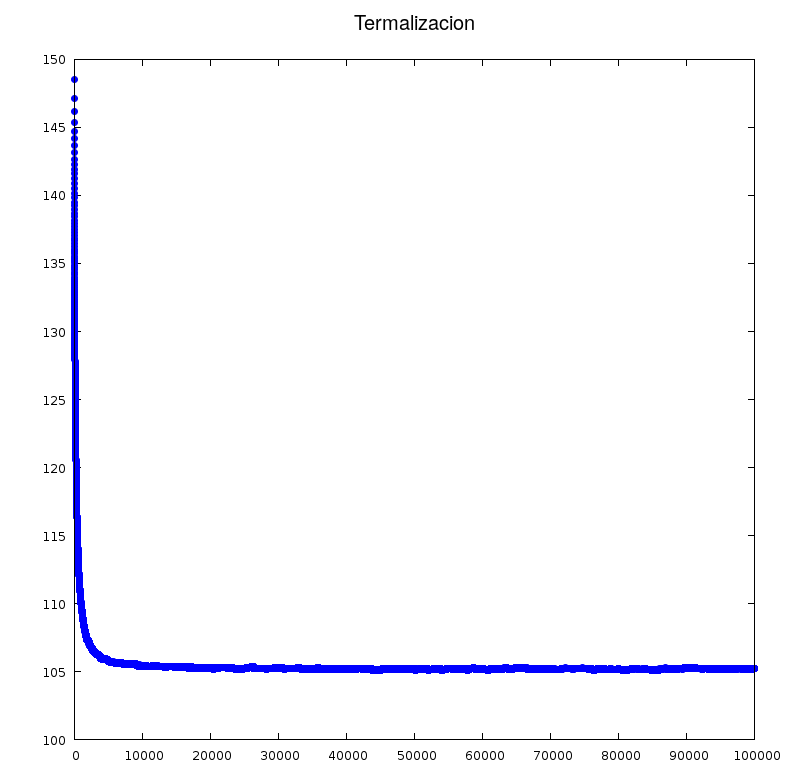
\includegraphics[width=0.75\linewidth]{Termalizacion.png}
	\caption{Curva de Termalizacion. Se utilizó un Potencial Yukawa}
	\label{CurvaTerma}
\end{figure}
A partir de esta curva podemos decir cuando el sistema se encuntras en equlibrio, lo que nos permite decidir en que punto comenzar a guradar configuraciones.

\subsection*{Configuraciones Inicial y Final}

Cuando se empieza, se genera una configuracion inicial aleatoria sin traslapes, el sistema conto con 800 particulas y una fración en volomen de $4.4\times 10^{-4}$ que aproxima a una concentracion de  $n^* = 8.40338122\times 10^{-4}$. Este ultimo es parametro de Gaylor. La celda era una caja cuadrada de lado $l=98.3736267$

Las configuraciones inicial y final fueron:
\begin{figure}[H]
	\centering
	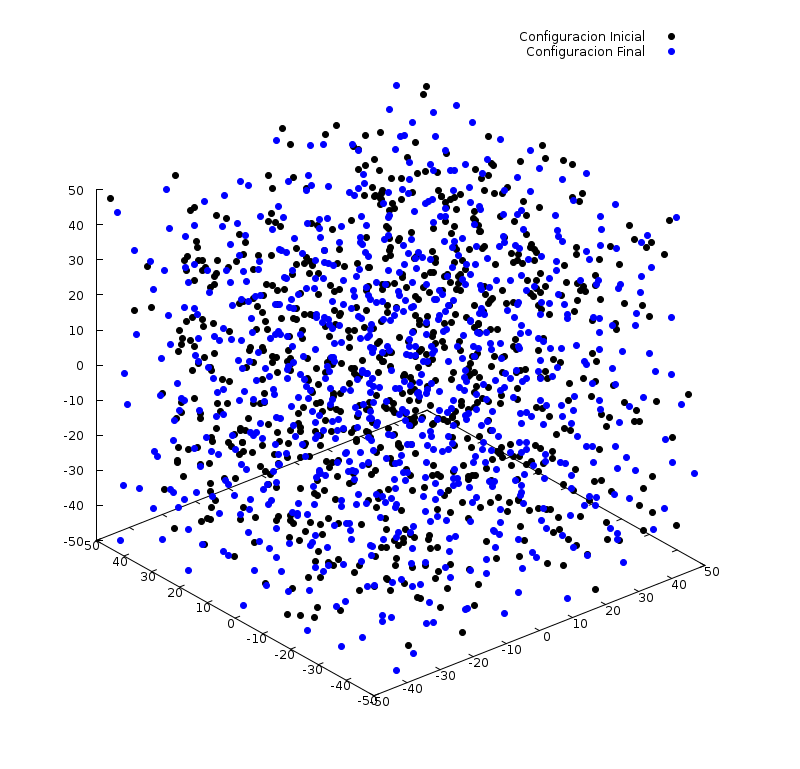
\includegraphics[width=0.75\linewidth]{Configuraciones.png}
	\caption{Configuración Inicial (Negro) y configuración Final (Azul)}
	\label{Configs}
\end{figure}

\subsection*{Función de distribución radial G(r)}
La simulación contó con $100,000$ configuraciones y guardo cada $100$ a partir de la configuración $20,000$ que fue caundo se considero que ya alcanzó el equlibrio. Se observa en la figura \ref{gdr} que aproximadamente cuando se alcanza $r\approx 7.5$ se empiezan a encontrar las partículas. Para cuando $r\approx 10.0$ este alcanza su máximo. En la figura \ref{gdr_Comp} se compara la G(r) de Gabriela con la propia.  Se observa que ambas se parecen, solo que la de gabriela presenta mas ruido. Esto se puede deber a que se uso un tamaño de cinta mas fino.

\begin{figure}[H]
	\centering
	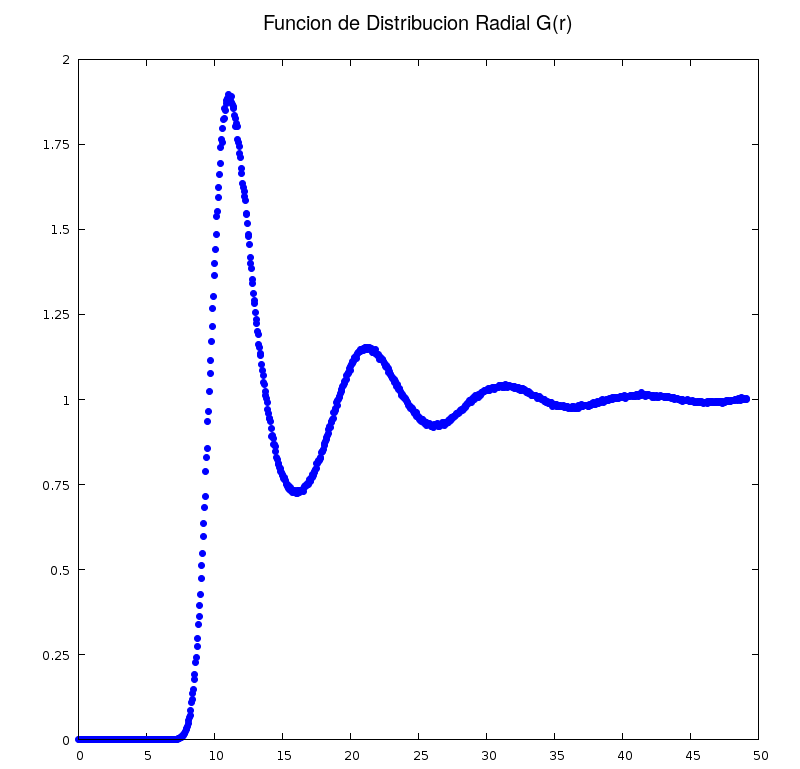
\includegraphics[width=0.75\linewidth]{gdrMartin.png}
	\caption{Funcion de Distribucion Radial de 800 particulas y $n^* = 8.4033\times 10^{-4}$ }
	\label{gdr}
\end{figure}
\begin{figure}[H]
	\centering
	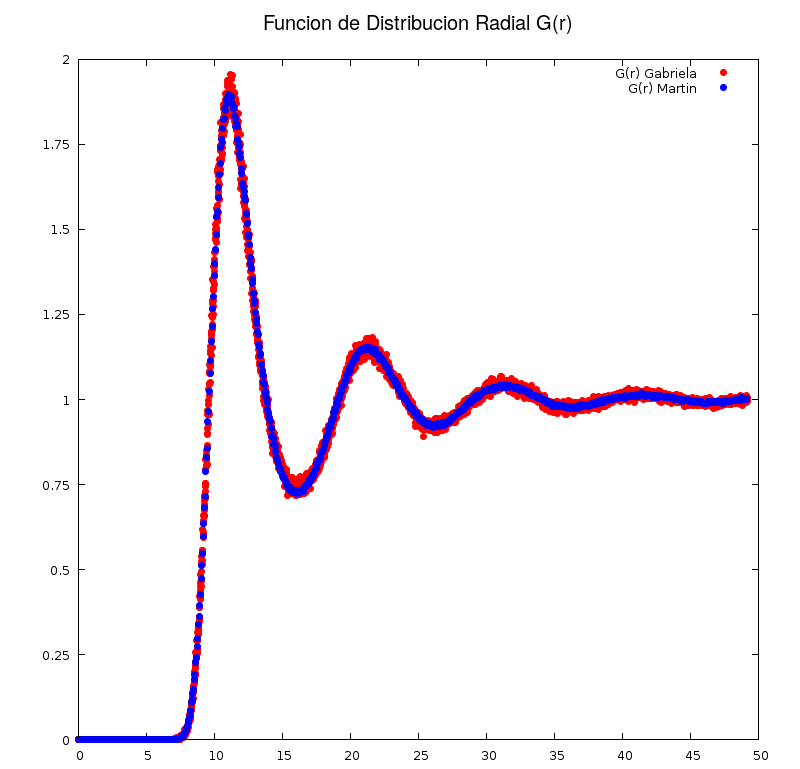
\includegraphics[width=0.75\linewidth]{GdrComparacion.png}
	\caption{Funcion de Distribucion Radial de 800 particulas y $n^* = 8.4033\times 10^{-4}$, Comparando con Gabriela}
	\label{gdr_Comp}
\end{figure}

\subsection*{Presión}
En este caso se pudo monitorear la presión del sistema conforme este evoluciono. Se obtuvo lo siguiente:

\begin{figure}[H]
	\centering
	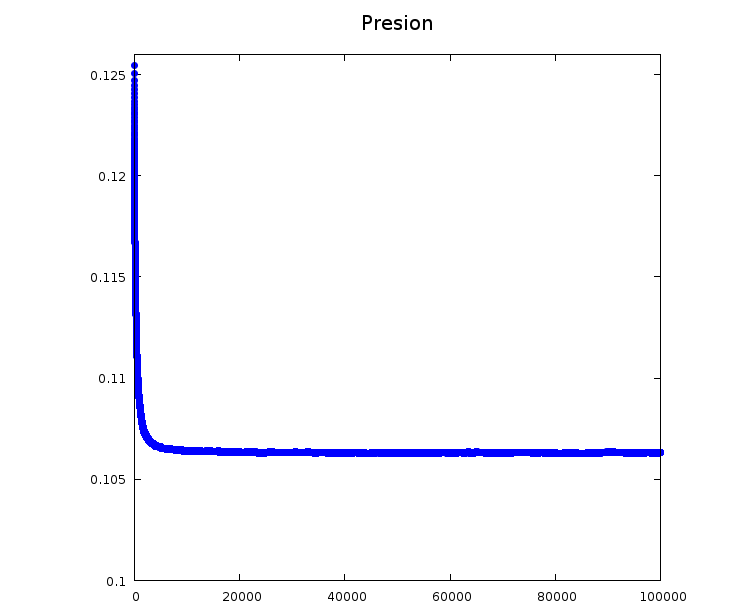
\includegraphics[width=0.75\linewidth]{Presion.png}
	\caption{Presión del sistema conforme este evoluciona}
	\label{Press}
\end{figure}



\subsection*{Código}
El codigo que se utilizo el fue le siguiente
\lstinputlisting[caption={Modulo de Variables Globales}]{Mod.f03}
\lstinputlisting[caption={Código Principal}]{Main.f03}
\lstinputlisting[caption={Código para generar la configuración Inicial Aleatoria}]{ConfigIni.f03}
\lstinputlisting[caption={Código para calculo de Fuerzas Potencial Yukawa}]{Fuerzas.f03}
\lstinputlisting[caption={Código para el calculo de la G(r)}]{GDR.f03}
\lstinputlisting[caption={Código del calculo de la W(t) y D(t)}]{WDT.f03}
\lstinputlisting[caption={Código para generar valores aleatorios con distribución gaussiana}]{RanGauss.f03}

\end{document}

